\documentclass{pre-tfg}

\usepackage{listings}
\usepackage{formular}
\usepackage[pdftex]{graphicx}
\usepackage{hyperref}
\usepackage{todonotes}

\showhelp  % comenta o borra para eliminar ayudas

\title{(TITLE)}
\author{María González Gutiérrez}
\docdate{(MONTH)}{2020}


\DeclareGraphicsExtensions{.pdf,.png,.jpg}

\usepackage{color}
\definecolor{gray97}{gray}{.97}
\definecolor{gray75}{gray}{.75}
\definecolor{gray45}{gray}{.45}

\lstset{ frame=Ltb,
     framerule=0pt,
     aboveskip=0.5cm,
     framextopmargin=3pt,
     framexbottommargin=3pt,
     framexleftmargin=0.4cm,
     framesep=0pt,
     rulesep=.4pt,
     backgroundcolor=\color{gray97},
     rulesepcolor=\color{black},
     %
     stringstyle=\ttfamily,
     showstringspaces = false,
     basicstyle=\small\ttfamily,
     commentstyle=\color{gray45},
     keywordstyle=\bfseries,
     %
     numbers=left,
     numbersep=15pt,
     numberstyle=\tiny,
     numberfirstline = false,
     breaklines=true,
   }

% minimizar fragmentado de listados
\lstnewenvironment{listing}[1][]
   {\lstset{#1}\pagebreak[0]}{\pagebreak[0]}

\lstdefinestyle{consola}
   {basicstyle=\scriptsize\bf\ttfamily,
    backgroundcolor=\color{gray75},
   }

\lstdefinestyle{C}
   {language=C,
   }


\renewcommand*\lstlistingname{Listado}



\begin{document}

\maketitle
\tableofcontents

\newpage


\section{INTRODUCCIÓN Y OBJETIVOS}


\section{FANFICTION, ARCHIVE OF OUR OWN Y RELATOS A UTILIZAR}
Un fanfic (abreviatura de “fanfiction”, “ficción del fan”) es una historia basada en una historia ya existente. Son, en esencia, historias creadas sin ánimo de lucro por los fans de un libro, película o videojuego. 
Crear fanfiction, en general, consiste en explorar temas e ideas que uno siente que faltan en la historia original. Puesto que cada fan tiene una interpretación distinta de los personajes y el mensaje que la historia original transmite, el fan convertido en autor puede añadir o quitar a la historia original lo que considere oportuno para contar su propia visión. Esto significa que cada fanfic es efectivamente una “transformación” de la historia original.
El fanfic cae en una zona gris en términos de derechos de autor, pero suele considerarse “fair use”. A día de hoy, la mayoría de fanfics se publican en sitios web de toda índole, destacando entre ellos \href{archiveofourown.org}{Archive Of Our Own}, que es un archivo open-source y sin ánimo de lucro creado expresamente para alojar obras creadas por fans. Según sus datos de mayo de 2020, tiene más de dos millones de usuarios registrados y más de seis millones de trabajos alojados. En particular elegí descargar los fanfics basados en \textit{Good Omens}, un libro de Terry Pratchett y Neil Gaiman, tanto por la cantidad de relatos existente como por mi familiaridad con esa comunidad.

Además de la cantidad y variedad de relatos que aloja, los motivos por el que elegí extraer los datos de Archive Of Our Own son su herramienta de búsqueda y filtrado, su sistema de etiquetas y el hecho de que permite descargar el archivo en HTML. Archive Of Our Own permite filtrar fanfics según varios parámetros y genera un enlace a ese subconjunto de relatos particular, muy útil para descargar una gran cantidad de datos.


\section{RECOGIDA DE FANFICS USANDO LA BASE DE DATOS DE ARCHIVE OF OUR OWN}

En el momento en el que decidí utilizar los fanfics de \textit{Good Omens} para el proyecto, dicho libro tenía unos 22000 fanfics en \href{archiveofourown.org}{Archive Of Our Own} (AO3 para abreviar). Sin embargo, de todos esos relatos sólo me interesaban los que están en inglés y los que realmente contuvieran texto (puesto que, aunque AO3 se centra en texto, permite todo tipo de archivos multimedia), de modo que utilicé el sistema de filtrado del sitio para seleccionar sólo los fanfics en inglés y que no estuvieran etiquetadas como "fanart", "podfic", etc, ya que indican que la obra no tiene texto. Tras este filtrado, quedaron 20190 relatos.

AO3 crea un enlace que lleva siempre a ese subconjunto de relatos, al cual puedo enviar peticiones HTTP GET y navegar las páginas. Cada página contiene un máximo de 20 fanfics, y antes de descargarlos es necesario llevar a cabo un segundo filtrado para evitar las obras sin texto que no hayan sido etiquetadas como tal por su autor. Decidí crear dos \textit{scrapers} distintos, uno para navegar por las páginas, filtrar y guardar los \textit{links} en un archivo, y otro que simplemente lee dicho archivo y realiza descargas.

\begin{itemize}
	\item El primer \textit{scraper} envía peticiones a AO3, explora el HTML de cada página para encontrar los objetos que encapsulan la información de cada fanfic, selecciona aquellos que tengan al menos 40 palabras por capítulo y crea una lista con los enlaces, que guarda en un archivo \textit{txt}.
	\item El segundo \textit{scraper} recorre los enlaces de dicho archivo y los descarga en una carpeta del sistema. Está hecho de tal manera que se le puede indicar qué tramo de la lista tiene que descargar (por ejemplo, del número 5000 al 6000).
	
\end{itemize}

Ambos \textit{scrapers} se encontraban de vez en cuando con el error 429 (Too Many Requests) y el 404 (Page Not Found). Se capturan fácilmente con un \textit{try-catch} que detecta el status de la página; para el 429 simplemente lanza una espera de dos minutos tras la cual reanuda su ejecución por donde la dejó, y para el 404 simplemente pasa a la siguiente, pues este error indica que el autor ha borrado su obra de la página y ya no está accesible.
 
Decidí dividir este proceso en dos programas (el de navegación y filtrado, y el que únicamente descarga) en vez de hacerlo todo en uno porque descargar los más de 20000 archivos de una vez lógicamente tardaría varias horas, y pensé que sería más pragmático si ejecuto una vez el \textit{scraper} crea una lista de enlaces, y luego ya ejecuto todas las veces que sean necesarias el \textit{scraper} que descarga, descargando cada vez un tramo distinto de la lista. De esta forma, pude descargar todos los fanfics en grupos de 2000 (alrededor de una hora y media), pudiendo tener el ordenador libre el resto del tiempo.

El poder ejecutar varias veces el segundo \textit{scraper} sin tener que volver a empezar desde el principio también demostró ser útil para lidiar con errores de red.

Ambos \textit{scrapers} utilizan la librería bs4 y BeautifulSoup para descargar y manejar los archivos HTTP. El resultado de su ejecución es una carpeta con 818,8 MB de archivos HTML.

\section{LIMPIEZA DE DATOS}

\section{ALGORITMO DE IDENTIFICACIÓN DE ENTIDADES}
Archivos encargados de realizar la identificación de entidades con nombre (NER, por el inglés) en los textos:
\begin{enumerate}
	\item POS\_tagger.py: para poder etiquetar las entidades nombradas es necesario etiquetar cada palabra con su rol morfológico, de modo que este programa se encarga de abrir los archivos html, pasarlos a texto y ponerle sus etiquetas morfológicas. Para ello utiliza los métodos de NLTK word\_tokenize y sent\_tokenize para dividir cada texto en frases y palabras, y pos\_tag para usar el clasificador por defecto de python para asignar etiquetar morfológicas en inglés. Almacena el resultado en un csv, de modo que en vez de tener preparar el archivo html y etiquetarlo cada vez que quiera identificar entidades, sólo tengo que etiquetar cada archivo una vez.
	\item NER\_trainer.py: entrena el algoritmo identificador de entidades usando el dataset de entrenamiento (descargado de aquí) y guarda el objeto en un archivo binario usando la librería pickle. Una vez entrenado, evalúa la precisión del algoritmo y la imprime por pantalla. Como el dataset no es parte del corpus nativo de NLTK, mucho de éste programa consiste en abrir el csv del dataset y empaquetar sus datos en listas y tuplas que sean compatibles con NLTK, y dividir el resultado en un dataset de entrenamiento y dos para hacer test (80\%, 10\% y 10\% del dataset original, respectivamente). Este programa utliza un objeto de la clase NERChunkerv1, que se encuentra en el archivo NER\_chunker.py, que se explica más abajo.
	\item NER\_tagger.py: utliza la libraría pickle para deserializar el archivo binario entrenado por NER\_trainer.py, y lo utiliza para etiquetar entidades nombradas en frases (usando etiquetas IOB). Utiliza el archivo csv creado por POS\_tagger para saltarse la parte de asignar etiquetas morfológicas, y guarda sus etiquetas en otro csv, de modo que gran parte de su código se dedica a lidiar con abrir, leer y actualizar archivos csv.
\end{enumerate}


Para manejar los archivos HTML utilizo \textit{BeautifulSoup}, y para los archivos csv utilizo pandas.
El código que propiamente contiene la lógica para la identificación de entidades se encuentra en NERChunker.py y está basado en este tutorial. NLTK llama ‘chunker’ a los algoritmos que dividen un texto en trozos de forma que no se solapen entre sí, y ‘tagger’ a los que ponen etiquetas. Así que en este programa hay dos clases, una que he llamado “NERChunkerv1” (en realidad tres, NERChunkerv1, v2 y v3. Hice varias para ver cuál iba mejor; la v1 es la que acabado utilizando) y otra que es “NERTagger”. También tiene dos funciones aparte, “feature\_fuction” y “word\_shape”, que son necesarias para NERTagger.

En NERChunkerv1 he utilizado una interfaz de NLTK llamada ChunkParserI. Tiene el constructor y dos métodos:
\begin{itemize}
	\item el constructor recibe el dataset en forma de frases etiquetadas y entrena el algoritmo. El dataset que he utilizado venía con etiquetas IOB en forma de tuplas, pero NLTK usa las etiquetas IOB en otro formato, de modo que el constructor se dedica principalmente a manipular las tuplas y aplicarles el método tree2conlltags para que NLTK las entienda. Y después llama a NERTagger y le pasa el dataset ya preparado para entrenar un clasficador.
	\item parse, que es el método que recibe una frase con etiquetas morfológicas y la etiqueta, con el clasificador ya entrenado. Devuelve la frase etiquetada con etiquetas IOB en forma de árbol, que es el formato de etiqueta que NLTK utiliza.
	\item evaluate, que evalúa la precisión del algoritmo. Uso el de la superclase, así que en mi código no está definido.
\end{itemize}


En NERTagger he utilizado una interfaz de NLTK llamada TaggerI, de los cuales defino dos métodos:

\begin{itemize}
	\item el constructor, que recibe el dataset de entramiento preparado por NERChunkerv1. Este dataset viene con etiquetas morfológicas y etiquetas IOB. Como queremos entrenar el clasificador para asignar etiquetas IOB a frases que nunca ha visto, las etiquetas morfológicas se consideran características de las palabras que lo acompañan. Primero hay que aplicar la feature function a cada palabra de la frase, cuya salida es un diccionario llamado “featureset” y después se prepara una lista de tuplas (featureset, tag) para entrenar un clasificador usando el algoritmo megam, que utiliza un modelo de maximización de entropía (maximum entropy model?). Para usar megam es necesario instalar a parte el modelo y configurar NLTK para que encuentre su path.
	\item tag, que es el método que recibe una frase con etiquetas morfológicas y la etiqueta con etiquetas IOB, con el clasificador ya entrenado. Aplica la feature fuction a cada palabra de la frase y la etiqueta con el clasificador.
\end{itemize}

Ambos métodos de NERTagger mantienen un historial de etiquetas IOB (una lista) y dependen de feature\_function, una función que recoge ciertas características (featureset) de una palabra y las devuelve en forma de diccionario. Las características que recoge son éstas:

\begin{enumerate}
	\item la palabra en sí
	\item la raíz de la palabra, usando un stemmer de NLTK llamado SnowballStemmer
	\item la forma de la palabra, que llama a una función auxiliar word\_shape, que consiste en una lista de expresiones regulares para determinar la forma de la palabra: number, punct, capitalized, allcaps, alllower, camelcase, mixedcase, wildcard, dot-end, abbreviation, hyphenated u other.
	\item La etiqueta morfológica asociada a esta palabra
	\item la palabra anterior a ésta
	\item la raíz de la palabra anterior
	\item la forma de la palabra anterior
	\item la etiqueta morfológica asociada a la palabra anterior
	\item la palabra anterior a la anterior
	\item la raíz de la palabra anterior a la anterior
	\item la forma de la palabra anterior a la anterior
	\item la etiqueta morfológica de la palabra anterior a la anterior
	\item la etiqueta IOB de la palabra anterior
	\item la etiqueta IOB de la palabra anterior a la anterior
	\item la palabra siguiente a ésta
	\item la raíz de la palabra siguiente
	\item la forma de la palabra siguiente
	\item la etiqueta morfológica de la palabra siguiente
	\item la palabra siguiente a la siguiente
	\item la raíz de la palabra siguiente a la siguiente
	\item la forma de la palabra siguiente a la siguiente
	\item la etiqueta morfológica de la palabra siguiente a la siguiente
\end{enumerate}

Algunos problemas encontrados mientras hacía estos programas:
\begin{itemize}
	\item Familiarizarme con la biblioteca NLTK, ya que nunca la había utilizado
	\item Mi conjunto de textos está en inglés pero NLTK no dispone de ningún corpus para entrenar NER en inglés, de modo que tuve que buscar un corpus ajeno, y hacer compatible sus etiquetas con el formato que NLTK utiliza (ambos utilizan etiquetas IOB, pero uno utiliza tuplas mientras que el otro usa árboles)
	\item descargar el modelo matemático megam y configurar python para que NLTK pueda utilizarlo.
	\item crear una feature function con los features adecuados, utilizando expresiones regulares para reconocer la “forma” de las palabras analizadas
	\item Debido a que el algoritmo necesita unas 2 horas para entrenarse, se utilizó la librería pickle para guardar el objeto y no perder el tiempo cada vez que se necesite ejecutar el algoritmo
	\item NLTK utiliza una estructura de datos tipo árbol para etiquetar los datos. Para recuperar los grupos de palabras y sus etiquetas e introducirlas en un dataframe de pandas es necesario recorrer todo el árbol. Aunque son árboles de como mucho profundidad 2, actualizar el dataframe con cada recursión tardaba demasiado tiempo, con lo que al final tuve que ir guardando el resultado de cada recursión en una lista y después guardar cada miembro de la lista en el dataframe. Descubrir la forma de “traducir” los árboles de NLTK a algo que el dataframe pudiera entender también tuvo su misterio.
	\item los archivos HTML de los fanfics, además de contener el texto, también contienen notas del autor, prefacios, resúmenes y metadatos sobre la historia, el autor y el sitio web que no me interesan para este trabajo, por lo que muchas funciones en POS\_tagger se dedican a eliminarlos.
\end{itemize}

\section{EVALUACIÓN DEL SISTEMA}

\section{RECOMENDACIONES}

Aquí habría que insertar tantas secciones como el alumno considere.

A continuación se indican una serie de recomendaciones que seguidas mejorarán la calificación final del trabajo.

\begin{itemize}
 \item Agrupar párrafos. La división del texto en múltiples párrafos independientes de pequeña longitud dificulta la lectura continua del documento.
\item  Evitar abusar de las listas con viñetas y las enumeraciones.
\item Utilizar un máximo nivel de profundidad secciones de 3 (hasta 3.1.1). Si se hace necesario una división más baja, no hacerlo con enumeración de subsecciones sino con texto en negrita y/o subrayada que represente el comienzo de cada subsección. 
\item  Si no hay más de una sección en un nivel no crearla. Es decir, si no hay al menos una 3.2 no crear la 3.1, ya que no tendría sentido dividir la sección 3.
\item  Utilizar referencias absolutas numéricas a tablas, figuras, secciones, etc. Por ejemplo: en la "Figura 3, se muestra el gráfico que  ..."; "Los resultados finales se encuentran en la Tabla X". Usar los ref y labels para que se actualicen las numeraciones automáticamente. No se debe hablar de ``en la siguiente figura'', ¿Qué pasa si reordeamos el texto o lo hace látex de manera automática?.
\item Cuando se referencia a una tabla, figura, sección, etc. hacerlo con la primera letra en mayúscula, ``En la Sección 1 ...''
\item  El texto siempre debe tener una alineación justificada. 
\item En el inicio de cada sección se debe hacer una breve introducción de lo que contiene y al final, unas pequeñas conclusiones y si es posible un texto de pequeña longitud que una con el siguiente capítulo.
\end{itemize}


\subsection{Inserción de Imágenes}

\begin{figure}[!h]
\centering
   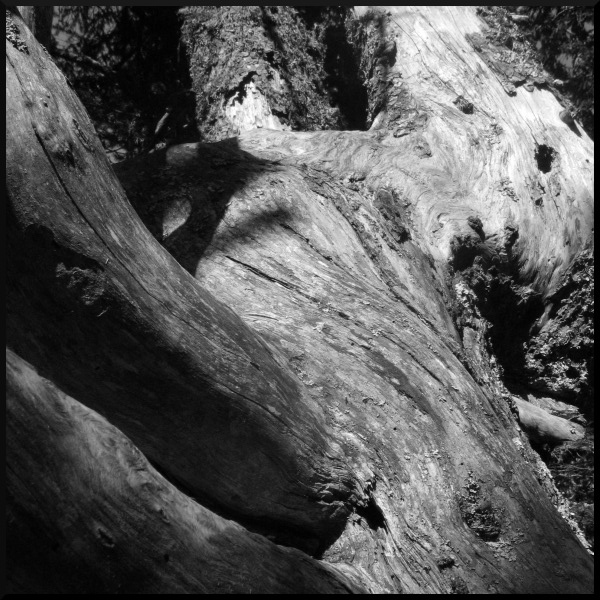
\includegraphics[width=8cm]{figures/tree04.jpg}
\caption{Árbol antiguo}
\end{figure}

\subsection{Inserción de órdenes de línea de comandos}

\begin{listing}[style=consola, numbers=none]
 gcc  -o e21 e21.c
\end{listing}





\subsection{Inserción de Código}

\begin{lstlisting}[caption=Ejemplo de código,style=C]

##include <stdio.h>
#include <sys/types.h>
#include <unistd.h>
#include <stdlib.h>

int main(void){

int register i;
int numHijos=4;
pid_t childpid;

for (i=0;i<numHijos;i++)
  if (childpid=fork()==0){
    sleep(1);
    printf("Proceso %ld con padre %ld\n", (long)getpid(), (long)getppid());
    exit(0);
  }

printf("Soy el proceso padre %ld\n", (long)getpid());
return 0;
}
\end{lstlisting}




\section{MEDIOS QUE SE PRETENDEN UTILIZAR}

\subsection{Medios Hardware}

El alumno deberá describir los medios hardware que prevé serán necesarios para el
desarrollo del proyecto.


\subsection{Medios Software}

El alumno deberá describir los medios software (lenguajes, entornos de desarrollo,
herramientas de gestión y planificación, etc.) que prevé serán necesarios para el
desarrollo del proyecto


\section{REFERENCIAS}

En esta sección se incluirán todas las referencias bibliográficas, ordenadas
alfabéticamente por el primer apellido del primer autor, de las obras de las cuales se
haya realizado alguna cita en los apartados anteriores. Las referencias deberán contener
datos básicos como nombre y apellidos de los autores, título de la obra, evento al que
pertenece, páginas, fecha y lugar de celebración (si se tratara de artículos de congreso),
ISBN, editorial y ciudad (si se tratara de libro), nombre de revista, páginas, volumen y
número (si se tratara de revista), etc.

Se empleará un formato de referencia reconocido en el ámbito académico como
ACM\footnote{http://www.acm.org/sigs/publications/proceedings-templates}\footnote{http://www.cs.ucy.ac.cy/\~{}chryssis/specs/ACM-refguide.pdf}.
Otros formatos aconsejables son, por ejemplo, IEEE, AMA, APA y AMA.

A continuación una sección de «Referencias» con ejemplos de referencias con formato ACM para:

\begin{itemize}
\item Un artículo de revista~\cite{Bow93}.
\item Un informe técnico~\cite{Ding97}.
\item Un libro~\cite{Tavel07}.
\item Un capítulo de libro~\cite{Greiner99}.
\item Un artículo en las actas de un congreso~\cite{Frohlic00}.
\item Para una página web~\cite{Steele04} (con autores conocidos).
\item Para una página web~\cite{Oxygen} (con autores desconocidos).
\end{itemize}


\bibliographystyle{alpha}
\singlespacing
\bibliography{ejemplo}


\end{document}


% Local Variables:
% coding: utf-8
% mode: flyspell
% ispell-local-dictionary: "castellano8"
% mode: latex
% End:
